\section{Relationship between RI expansion and momentum transfers}
\begin{frame}
\frametitle{RI expansion and momentum transfers}
\begin{equation}
\hat{H}^{(2)}=\frac{1}{2 \Omega} \sum_{\mathbf{Q} \neq 0} \frac{4 \pi}{Q^2} \hat{\rho}^{\dagger}(\mathbf{Q}) \hat{\rho}(\mathbf{Q})
\label{eq:two_body_hamiltonian}
% \hat{H}^{(2)}  =\frac{1}{2} \sum_{\mathbf{Q}>0}\left[\hat{A}^2(\mathbf{Q})+\hat{B}^2(\mathbf{Q})\right]
\end{equation}
where 
\begin{equation}
\hat{\rho}(\mathbf{Q}) = \sum_{G , \lambda} c_{\mathrm{G}+\mathrm{Q}, \lambda}^{\dagger} c_{\mathrm{G}, \lambda}, \theta\left({E_{\text {cut }}-|\mathbf{G}+\mathbf{Q}|^2 / 2}\right), \lambda \in \alpha ,\beta .
% \overline{\rho(Q)} \equiv \sum_{G . \lambda} c_{\mathrm{G}+\mathrm{Q}, \lambda}^{\dagger} c_{\mathrm{G}, \lambda}, \theta\left(\overline{E_{\text {cut }}-|\mathbf{G}+\mathbf{Q}|^2 / 2}\right)
\end{equation}
\pause
For the UEG at $\Gamma $, $\bm{G}=\bm{G'}$ and $\bm{q}=0$, so $\bm{\epsilon}^{-1}_{\bm{G}\bm{G'}}(\bm{q},\omega)\rightarrow \bm{\epsilon}^{-1}(\bm{Q},\omega)$ 
\pause
and
\begin{align}
\bm{\epsilon}^{-1}(\bm{Q},\omega) &\overset{\text{TDL}}{=}\begin{bmatrix}
 1/{\tilde{B}}_{PP}(\omega) 
    \end{bmatrix}\\
   \bm{\epsilon}^{-1}(\bm{Q},\omega) &\overset{\text{fc}}{=}\begin{bmatrix}
      1/h_{00}(\omega)        & 0 \\
      0        & 1/{\tilde{B}}_{PP}(\omega) 
    \end{bmatrix}
\end{align}
\end{frame}

\section{PPMs vs. exact}
\begin{frame}
\frametitle{Satisfying the f-sum rule in a finite supercell}
\begin{align}
    \int_0^{\infty} d \omega \omega \operatorname{Im} \epsilon_{G G^{\prime}}^{-1}(\mathrm{q} ; \omega) &= -\frac{\pi}{2} \omega_p^2 \frac{\rho\left(\mathrm{G}-\mathrm{G}^{\prime}\right)}{\rho(0)} \frac{(\mathrm{q}+\mathrm{G}) \cdot\left(\mathrm{q}+\mathrm{G}^{\prime}\right)}{\mid \mathrm{q}+\mathrm{G}^2}\\
\implies \Omega_{G G^{\prime}}^2(\mathrm{q}) &= \omega_p^2
\end{align}
\pause
\begin{itemize}
  \item This is true for a $\epsilon^{-1}$ only in the TDL. \pause
  \item Idea: integrate fc $\bm{\epsilon}^{-1}$ numerically on a coarse frequency grid
\end{itemize}
\end{frame}
\begin{frame}
\frametitle{Inverse dielectric}
\begin{figure}
    \centering
    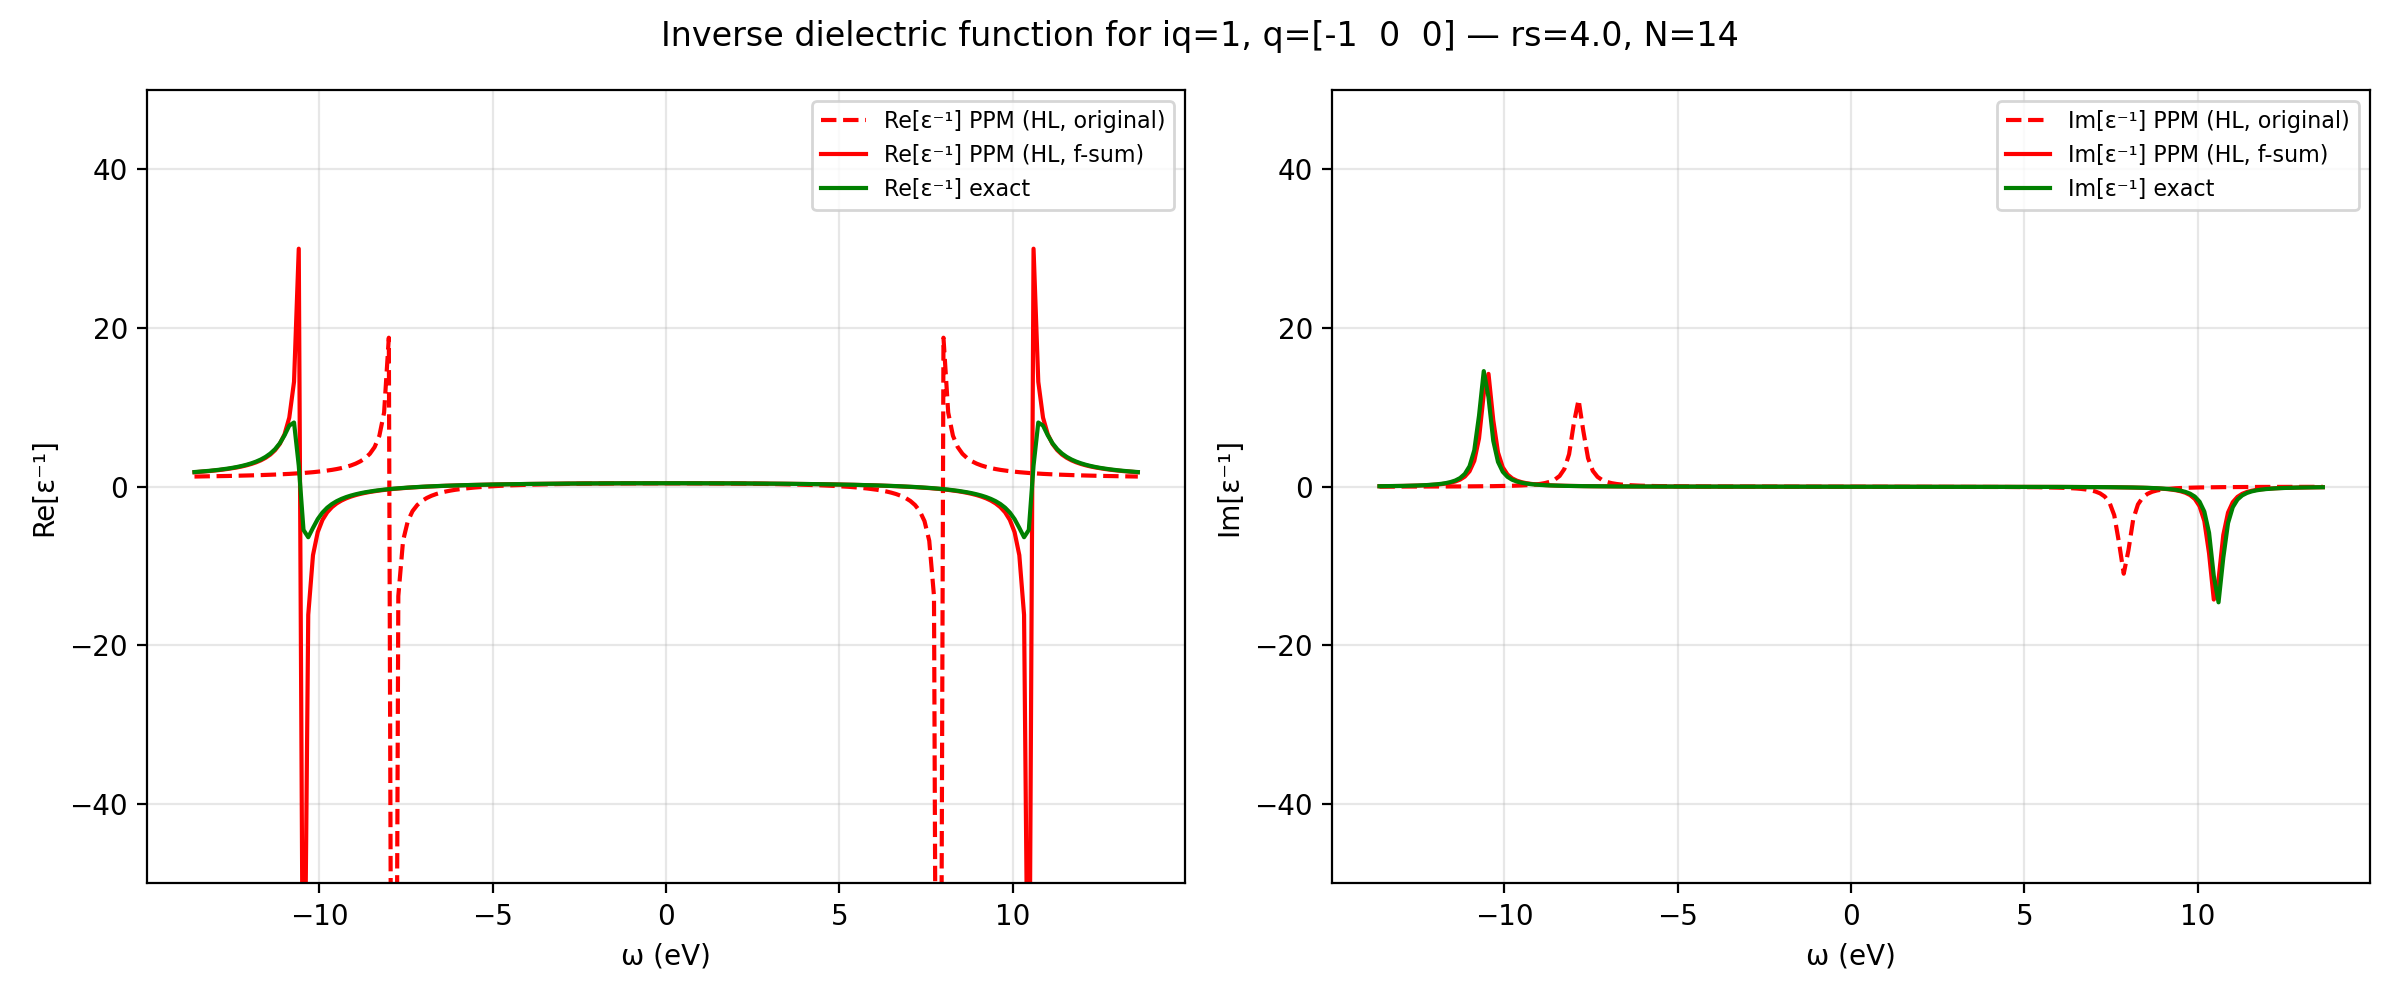
\includegraphics[width=\textwidth]{figs/dielec_5-14.png}
\end{figure}\pause
\begin{itemize}
  \item Compare with Literature
  \item using HL, fsum moving forward
\end{itemize}
\end{frame}

\begin{frame}
\frametitle{self energy}
\begin{figure}
    \centering
    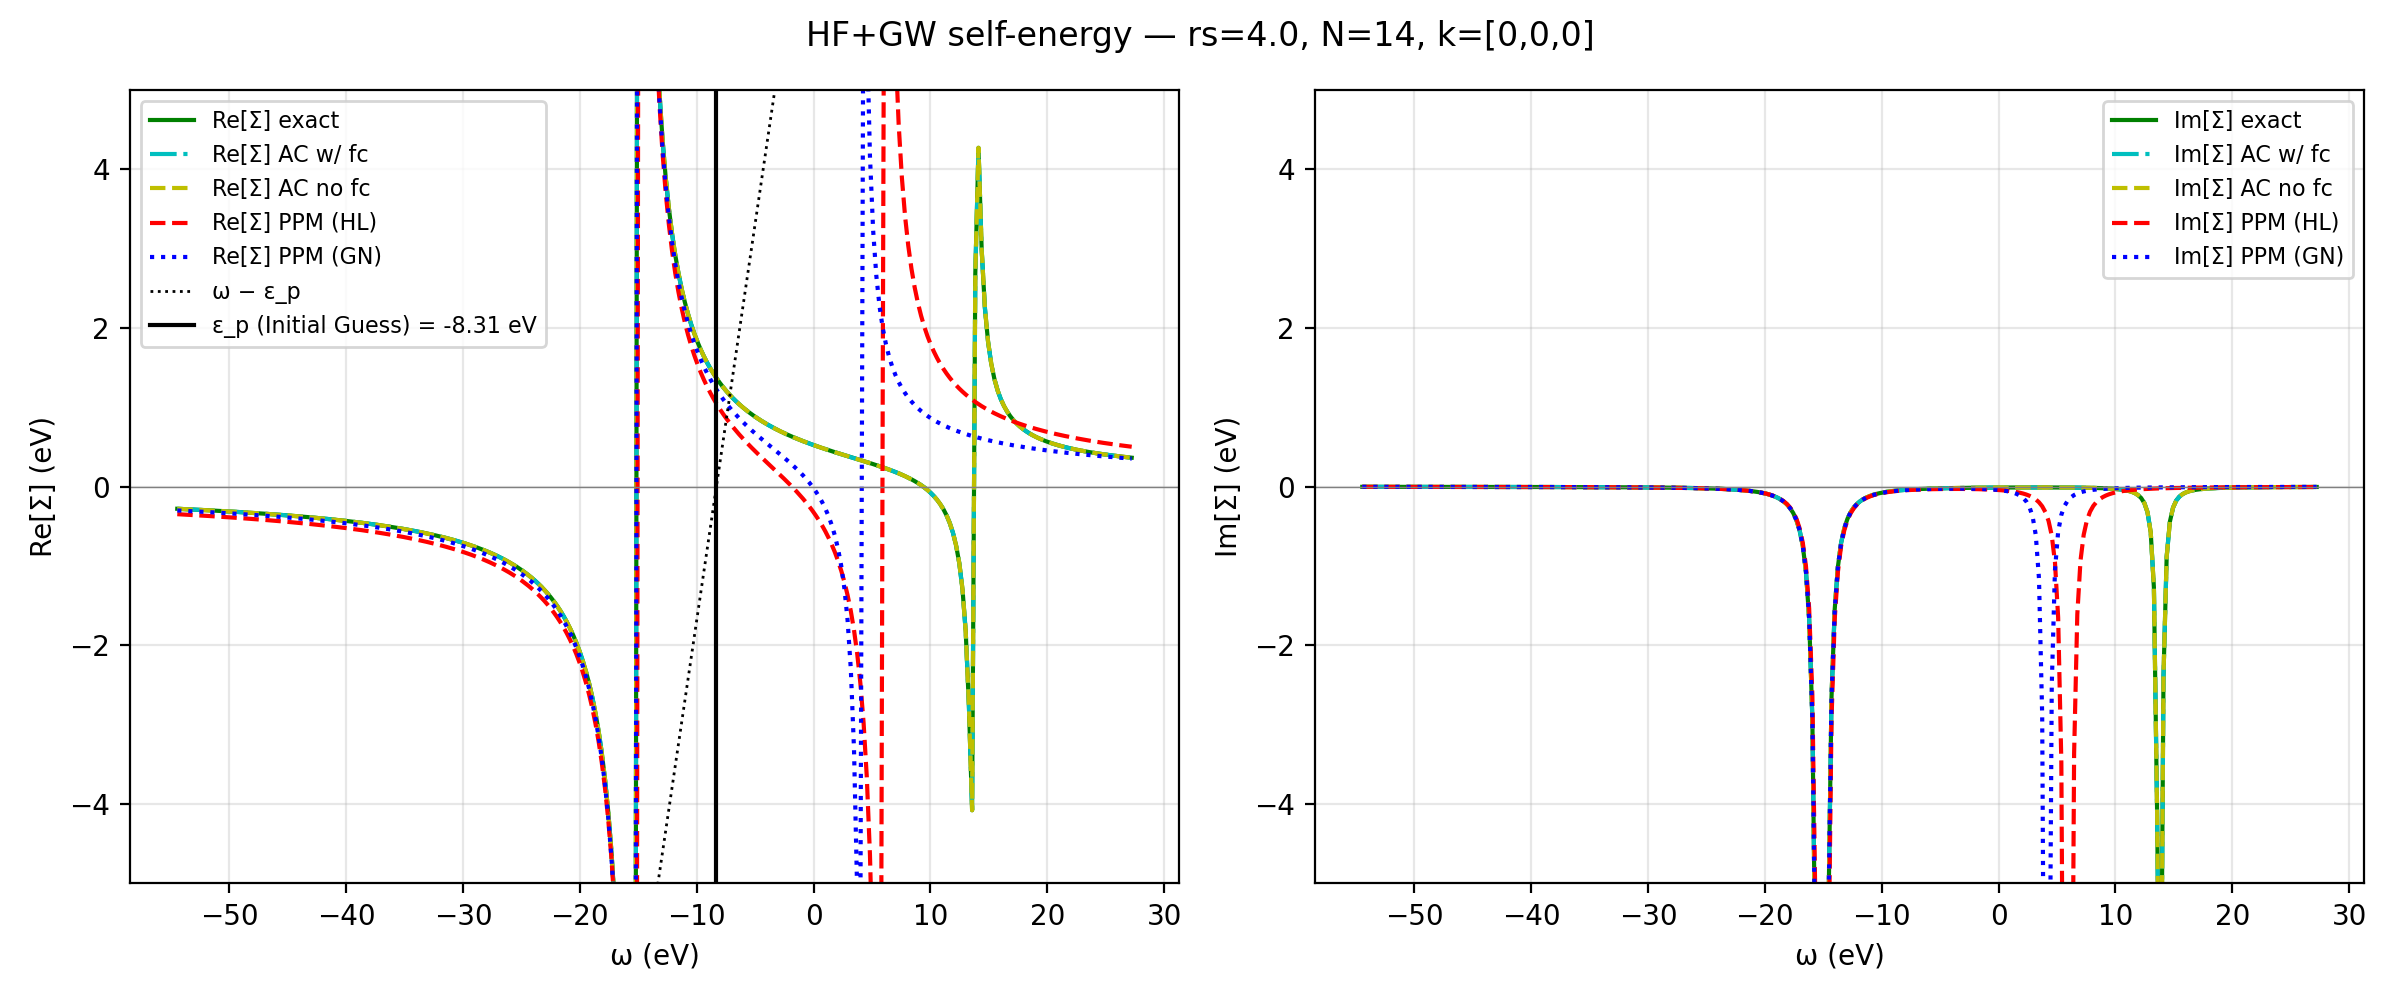
\includegraphics[width=\textwidth]{figs/sigma_5-15v2.png}
\end{figure}
\end{frame}
\begin{frame}
\frametitle{spectral function}
\begin{figure}
    \centering
    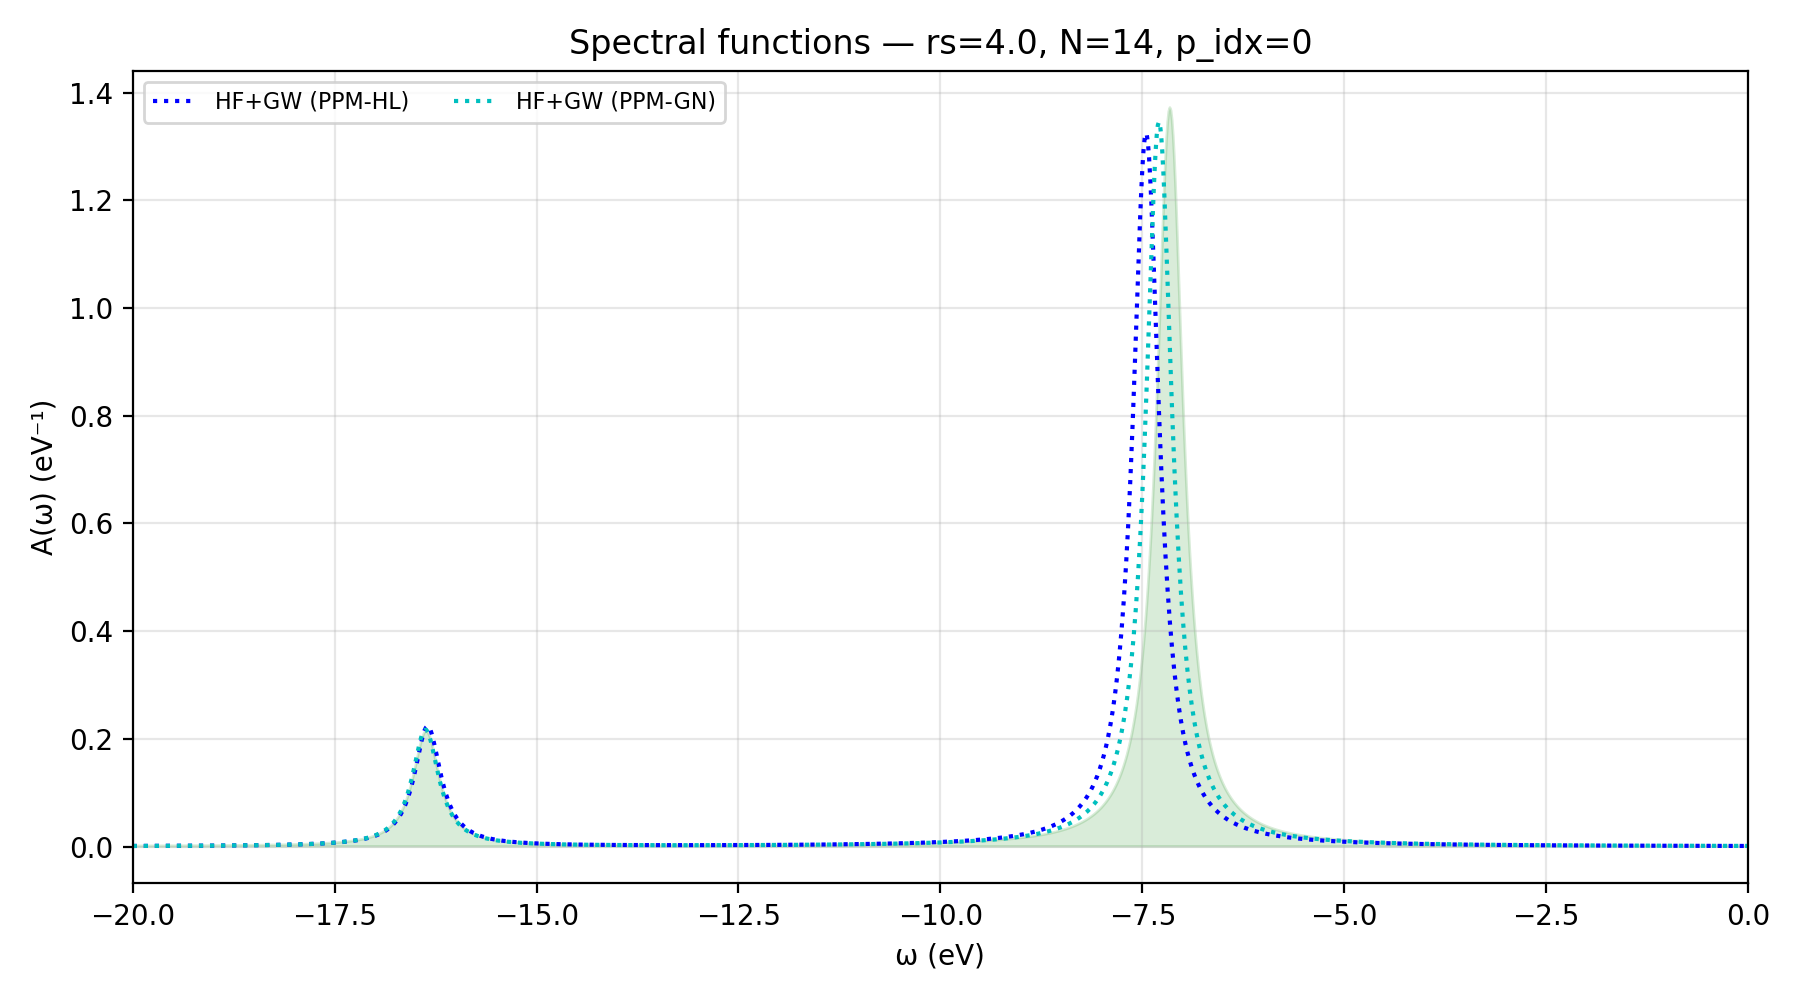
\includegraphics[width=\textwidth]{figs/spec_5-14.png}
\end{figure}
\end{frame}
\section{BWs2 ideas}
\begin{frame}
\frametitle{BWs2 ideas}
\begin{enumerate}
    \item Do we properly account for finite-size corrections in
  \begin{equation}
    C_{pp}^{\mathrm{BWs2}}(t) = 
    \frac{1}{2} \sum_{i a b}\frac{\langle p i \| a b\rangle^2 }{\left(\tilde{\varepsilon}_{p i}^{a b}\right)^2}
      \left(e^{-i \tilde{\varepsilon}_{p i}^{a b} t} + i \tilde{\varepsilon}_{p i}^{a b} t -1 \right) 
    + \ldots
  \end{equation}
via
\begin{align}
  \hat{H}^{(0)}&=\hat{H^{(0)}}+\frac{\alpha_1}{8}\left(t_{i k}^{a b(1)}\langle j k \| a b\rangle+t_{j k}^{a b(1)}\langle i k \| a b\rangle-\frac{2}{N} t_{k l}^{a b(1)}\langle k l \| a b\rangle \delta_{i j}\right) \hat{a}_i^{\dagger} \hat{a}_j + \ldots
\end{align}
\pause
\item Using BWs2 as AFQMC trial wavefunction
\pause
\item A more exhaustive exploration of the BWs2 Green's function
\end{enumerate}
\end{frame}
